\documentclass[10pt]{article}
\usepackage[margin=1in]{geometry}
\usepackage{indentfirst}
\usepackage{adjustbox}
\usepackage{listings}
\usepackage{color}
\usepackage{graphics}
\usepackage[hidelinks]{hyperref}
\usepackage{rotating}
\usepackage[final]{pdfpages}
\definecolor{dkgreen}{rgb}{0,0.6,0}
\definecolor{gray}{rgb}{0.5,0.5,0.5}
\definecolor{mauve}{rgb}{0.58,0,0.82}
\lstset{frame=tb,
	aboveskip=3mm,
	belowskip=3mm,
	showstringspaces=false,
	basicstyle={\small\ttfamily},
	numbers=none,
	numberstyle=\tiny\color{gray},
	keywordstyle=\color{blue},
	commentstyle=\color{dkgreen},
	stringstyle=\color{mauve},
	breaklines=true,
	breakatwhitespace=true,
	tabsize=3
}
\title{Return Value Testing of Linux Applications}
\author{Keith Funkhouser, Malcolm Reid, Colin Samplawski}
\date{Fall 2016}

\begin{document}
\setlength{\baselineskip}{18pt}
\maketitle

\begin{abstract}
\setlength{\baselineskip}{18pt}
We used fuzz testing methods to investigate the robustness of various Linux applications. We developed a mechanism to intercept system and library calls and return an error return code to the calling application. We defined crashes as unintentional core dumps or hangs. Of the 90 applications tested, we encountered crashes in 18 (20.0 \%) for at least one of the 22 calls we tested. We investigated the source code for some of these crashes and provide analysis in this paper. 
\end{abstract}

\section{Introduction}
Many commonly used C library functions return some value. In most cases, this value indicates something that is relevant to the  function's operations, such as a file descriptor, number of bytes processed, or a pointer to some data. Additionally, many functions that can fail return some predefined value indicating that an error occurred during the function's execution. Unfortunately, many programmers have the bad habit of not checking these return values for such error conditions, which can lead to undesirable behaviors, such as the program crashing or hanging. In our work, we used library interposition to intercept system and library calls in order to force an error value to be returned to an application probabilistically. In doing so, we were able to evaluate the robustness of these applications to returned error values.

Error handling takes many forms in the programs that were tested. For example, one of the simplest techniques (though not exactly considered the ``best practice'') is to simply \texttt{abort} on error, or \texttt{assert} that an error was not returned. We detected these situations based on the signal sent to kill the process. Although these are inelegant ways to terminate a program, nevertheless they are \emph{intentionally} performed by the programmer. Therefore, here we have used an expanded definition of robustness to mean that the program does not crash or hang. We define ``crash'' to mean an unintentional core dump (not brought about by the programmer) and ``hang'' to mean behavior that could only be ended by forcing the application to terminate. This narrower definition of misbehavior allowed us to quantify program behavior in an unambiguous way.

Nearly all of the applications we tested displayed aberrant behavior that is likely not what the developers intended, but this sort of behavior was too subjective for us to meaningfully measure. Nevertheless, we do include some of the more interesting aberrant behaviors that we found while testing.

In order to assess as large a representative sample of available programs as possible, we decided to focus on two major groups: small-scale (command-line) utilities, and large-scale (primarily GUI-based) programs. We restricted our sample to open-source projects, so as to be able to debug with source code available. Within small-scale utilities, we selected three subgroups to focus on: GNU Core Utilities (e.g. \texttt{ls}), the \texttt{net-tools} project (e.g. \texttt{ifconfig}), and selected other common utilities, such as \texttt{make} and \texttt{grep}. Within large-scale programs, we selected a sample of some of the largest and most common desktop programs available, such as Google Chrome, Mozilla Thunderbird, and \texttt{gcc}.


\section{Related Work and Motivation}
Pioneered by Miller et al. in 1990, fuzz testing is conducted by passing randomly generated input to applications in order to find bugs \cite{bartoriginal}. In that work, they used fuzz testing to assess reliability in UNIX applications by determining the number that crashed or hung when passed fuzzed input. Surprisingly, they found that 25-33\% of the applications tested crashed or hung. In a follow-up study in 1995, Miller et al. found that, although the programs that were tested in the previous study improved in reliability, almost 50\% of the programs tested crashed or hung \cite{bart}.

In this second study, rather than passing randomly generated data, they intercepted \texttt{calloc}, \texttt{malloc}, and \texttt{realloc} calls and returned an error value with some probability $p$. Here, we extend that work by expanding the scope of both the calls intercepted, and the number of programs tested. In addition to the memory allocation-related functions, we add file operation calls, \texttt{pthread}-related calls, and others. In addition to many of the same command-line utilities tested, we expand the scope to include larger-scale graphical programs and a number of other common small-scale utilities.

\section{Mechanisms}
We needed a way to intercept system and library calls made by an application in order to inject bad return values. The technique also needed to be difficult to detect, lest it be circumvented, and innocuous so that it would not disrupt the normal execution of the program apart from the return value given. Furthermore, it needed to be fine-grained enough so that only calls from the  application being tested would be intercepted, lest it crash our whole system.

\subsection{Library Interposition}
Using the environment variable \texttt{LD\_PRELOAD}, a user can specify a shared library object that is loaded before any others at dynamic linking time \cite{ldpreload}. Importantly, functions within this shared library take precedence over any other functions of the same name, even ones found in \texttt{libc} and other standard libraries.

\subsubsection{Benefits of LD\_PRELOAD}
\texttt{LD\_PRELOAD} affords several benefits to the amateur fuzz tester. Primarily, it is extremely simple to work with, and therefore difficult to get wrong: just set an environment variable and run the (dynamically linked) binary. We took this approach in order to test a greater number of calls and utilities as quickly as possible, but given more time we may have opted to use binary rewriting. Furthermore, this method enables the interception of calls many levels deep in the stack, even in other dynamically linked libraries. We perceive this to be a benefit, as programs which depend on shared libraries are taking on the risk that those libraries are written incorrectly.

\subsubsection{Limitations of LD\_PRELOAD}
There are several limitations to this method. Significantly, statically linked applications bypass our wrappers completely; however, we did not encounter any statically linked applications. Other approaches, such as the binary rewriting techniques used by Miller et al. \cite{bart} or a dynamic instrumentation tool such as DynInst \cite{dyninst}, circumvent this issue by modifying the binary directly, and would be necessary to expand coverage to statically linked programs.

Another limitation to our method is that it is Linux-specific. \texttt{LD\_PRELOAD} is found on many Linux distributions and some other UNIX systems, such as BSD \cite{bsd}. However, there are equivalents found on other popular systems such as the \texttt{AppInit\_DLLs} registry value on Windows \cite{dll} and the \texttt{DYLD\_INSERT\_LIBRARIES} environment variable on macOS \cite{macos}. Therefore, we feel confident that this methodology could find success when applied to applications on the most common commodity operating systems.

\subsubsection{Implementation}\label{ld_preload_implementation}
For each call of interest, we created a position-independent shared library object containing a single wrapper function with the name of the call. The wrapper simply returns an error value with probability $p$, or calls the real version of the function with probability $1-p$. In this way, we probabilistically either inject an error value, or allow the application to continue as usual. A visual representation of this mechanism is given in figure \ref{fig:ld_preload}. Each program of interest was tested with one call being intercepted at a time.

This probabilistic approach is used to attempt to test all of the calls to a given function within an application. If error values were returned 100\% of the time, we would not be able to evaluate program behavior on all possible code paths. For example, if a program calls \texttt{malloc} in two locations and crashes or aborts after an error value is returned from the first, then the second call will never be reached. To account for different program structures, we tested each call for each program on a variety of error return probabilities, ranging from 1\% to 50\%. Applications that make a particular call many times require a lower probability of returning an error in order to cover all possible code paths. Likewise, applications that make a particular call (e.g. \texttt{fork}) infrequently require a higher probability of returning an error in order to cover all possible code paths.
\begin{figure}
  \centering
	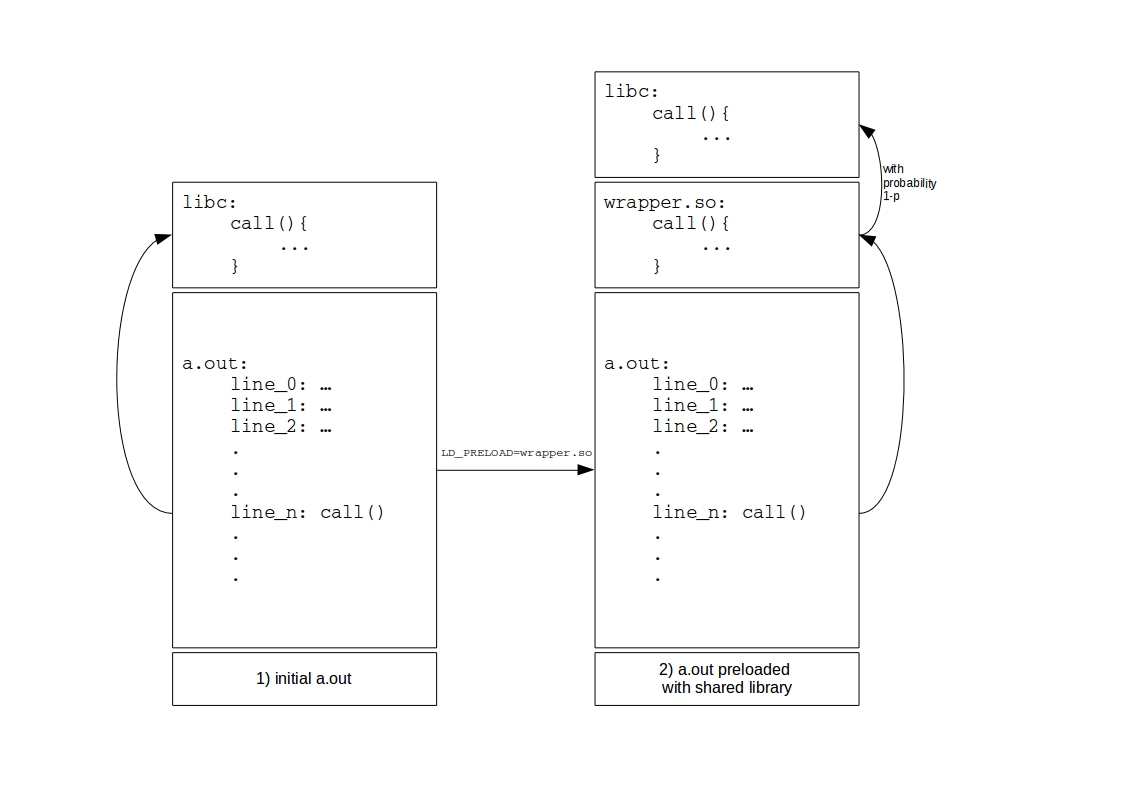
\includegraphics[width=0.8\textwidth]{ldpreload_fig}
	\caption{Library interposition allows for system and library calls to be overriden at runtime without recompilation or modification of the binary.}
  \label{fig:ld_preload}
\end{figure}

Returning the correct value from within a wrapped function is non-trivial: infinite recursion results if one attempts to invoke the same call that is being wrapped. To avoid the recursion, we used the \texttt{dlsym} function, which scans through the dynamically loaded libraries for a function that has the same name as the argument passed to it. Upon finding such a function, a function handle (that is, an address) is returned. This function handle can then be used in order to call the original version of the function. An example of such a wrapper is shown in the ``Generated Wrapper'' portion of Figure \ref{fig:codegen}.


\subsection{Wrapper Generation}
The wrappers described in section \ref{ld_preload_implementation} are uniformly structured: they contain one method, the signature of which is identical to that of the overridden call. Furthermore, nothing specific about the call's implementation is necessary for generating the wrapper. Thus, wrappers are good candidates for automatic code generation by inspection of the appropriate header files. For example, by examining the \texttt{stdlib.h} file and knowing one piece of information from the \texttt{MALLOC(3)} \texttt{man} page, we can completely construct the wrapper (Figure \ref{fig:codegen}).

\begin{figure}[h!]
\centering
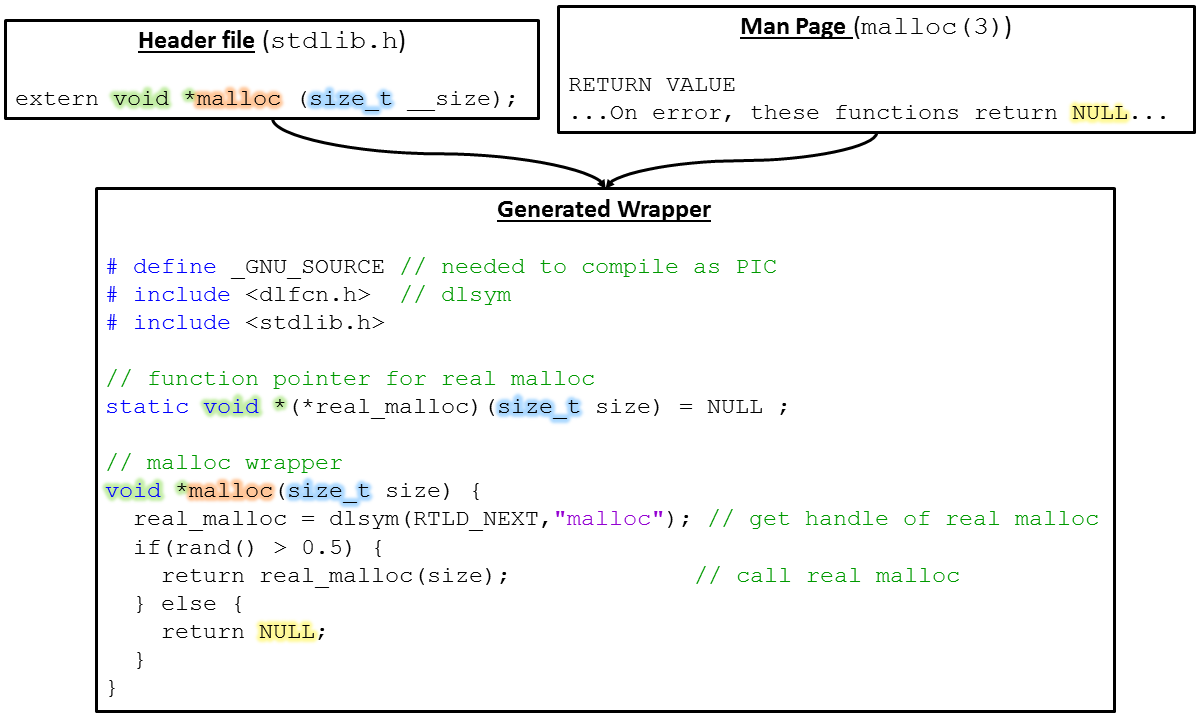
\includegraphics[width=0.8\textwidth]{codegen_figure}
\caption{Generation of wrappers is possible by parsing the abstract syntax tree of the appropriate header file and manually annotating the error value to be returned.}
\label{fig:codegen}
\end{figure}

We developed an input file which contained the call name, (error) return value, \texttt{errno} (if applicable), and the header file to be included in the wrapper (usually given at the top of the \texttt{man} page). Our script parsed this input file and generated the appropriate wrappers. The script uses the \texttt{pycparser} Python module \cite{pycparser} to traverse the abstract syntax tree derived from the header file.

This technique has several benefits, the primary one being that it reduces development time when wanting to make small changes to all of the wrappers. For example, after starting with a wrapper that simply returns the value of the real call using \texttt{dlsym}, we want to add a ``coin flip'', which simply determines at random whether to return the correct value or the error value. It is trivial to do this via code generation, by simply adding a few lines to the script and re-running it to update all of the downstream wrappers.

We are unsure whether the added development cost of this approach outweighs the potential speedup in development time. It is true that the wrapper files are only infrequently modified, however when dealing with almost 20 wrappers, it becomes increasingly tedious to make changes in a manual way. At the very least, we hope that these techniques are useful for others in the testing community.

\section{Command-line Utilities}
The main group of applications that we tested was comprised of small command-line utilities. Most of these are from the GNU Core Utilities project. As described by the Free Software Foundation, ``the GNU core utilities are the basic file, shell and text manipulation utilities of the GNU operating system." [?] These utilities were chosen because they represent some of the most commonly used applications on Linux systems. In addition to the GNU core utilities we included some other common utilities that are not part of the project. Listing 4 displays the utilities that we tested. For each of these utilities, we tested using each the calls in Listing \ref{lst:coreutils_wrappers}.

%The GNU Core Utilities project (henceforth ``coreutils'') is comprised of over 100 programs (many of them reimplementations of the original utilities found in UNIX) which provide basic file, shell, and text manipulation. Per their documentation, these are tools which are ``expected to exist on every [GNU] operating system'' \cite{coreutils}. As such, the robustness of these programs is of great importance, as they will be used by many users on a variety of systems.

%In order to assess the robustness of the coreutils programs when given error return values from a variety of calls, we selected 62 of the coreutils programs to test (listing \ref{lst:coreutils_progs}).

% table:

\iffalse
cat ~/ReturnValueTester/test\_dir/utils.txt.bak | egrep -v '^#|^$' | cut -d "|" -f 1 | sort > utils_used.txt
ls -f -a -1 ~/Downloads/coreutils-8.25/src/*.c | rev | cut -d "/" -f 1 | rev | cut -d "." -f 1 | sort > coreutils.txt 
comm utils_used.txt coreutils.txt -12 | column -c 80
\fi

\begin{lstlisting}[label={lst:coreutils_progs},caption={GNU Core Utilities tested}]
base64          dirname         logname         sort            uniq
basename        du              ls              stat            unlink
cat             echo            md5sum          sum             uptime
chmod           expr            mkdir           touch           users
cksum           factor          mktemp          tr              wc
comm            fold            mv              true            who
cp              groups          nproc           truncate        whoami
cut             head            printenv        tsort
date            hostid          pwd             tty
df              id              seq             uname
dircolors       link            shred           unexpand NOT TRUST THIS TABLE!
\end{lstlisting}



% ls -f -a -1 ~/ReturnValueTester/wrappers/*_wrapper.c | rev | cut -d "/" -f 1 | rev | cut -d "_" -f 1 | uniq | column -c 80
\begin{lstlisting}[label={lst:coreutils_wrappers},caption={Wrapped calls for testing Command-line Utilities}]
calloc  creat   execv   fork    malloc  opendir pipe    pthread_create 	realloc
close   execvp  fopen   fstat   mmap    open    poll    pthread_mutex	read    
write
\end{lstlisting}

We hypothesized that utilities of this type would yield very few crashes. The justification for this is two-fold. Primarily, the project is extremely mature: in 2002, the GNU fileutils, textutils, and sh-utils projects merged into the GNU coreutils project, but each of those three projects had a substantial development history at that point in time. In the same vein, the binaries from the coreutils project are used in production all over the world, and therefore are more well-tested than other open source projects. Additionally, these utilities have relatively few lines of code and total calls and are therefore easier to get correct.
 %Furthermore, we hypothesized that the most common source of errors would be from the \texttt{malloc} family of calls.

\subsection{Results}
Our results suggest that the coreutils project is extremely robust to error values returned from the calls tested. Namely, we were able to achieve crashes in two of the programs, \texttt{du} and \texttt{hostid}. Both of these crashes came through intercepting calls to \texttt{malloc}. See listings \ref{lst:du/malloc} and \ref{lst:hostid/malloc}.


\section{\texttt{net-tools}}
\subsection{\texttt{net-tools}}
The \texttt{net-tools} suite includes several small utilities that form the base of the networking distribution for Linux \cite{nettools}. We hypothesized that \texttt{net-tools} would yield a significant number of crashes or hangs, as some of the utilities in it have been deprecated in favor of the \texttt{ip} utility. We tested 11 utilities and found that 4 (36.4\%) crashed (table \ref{lst:net-tools}). \texttt{malloc} was the source of all of the crashes. A more detailed investigation into the root cause of some of these crashes is given in Appendix \ref{appendix:net-tools}.

\begin{table}[h]
\begin{tabular}{l}
\begin{lstlisting}
m dnsdomainname m ifconfig      m netstat         route
  domainname    m ipmaddr         nisdomainname   ypdomainname
  hostname        mii-tool        rarp
\end{lstlisting}
\end{tabular}
\caption{\texttt{net-tools} utilities tested; those which crashed with \texttt{malloc} are indicated with \texttt{m} to their left. A total of 4/11 (36.4\%) crashed.}
\label{lst:net-tools}
\end{table}

\section{Large-scale Programs}
In addition to the smaller utilities discussed above, we tested a collection of large-scale open source applications. Admittedly, we do not offer a well defined distinction between small and large-scale, but we loosely define large-scale as applications that are composed of substantial code bases and represent long term projects from major vendors. We believe that these applications are an important portion of our testing suite because they demonstrate the scale that modern applications can achieve today and could not in 1995 for Miller et al. Furthermore, we expected to find more crashes in applications of these types, following the common wisdom that larger programs are generally more difficult to get correct.


One difficulty in testing large-scale applications is determining the set of behaviors to test. Applications of this size offer a large set of features and many of these features do not have analogs in other applications. For example, gvim and LibreOffice offer document editing, while Firefox and Chrome offer no such analagous behavior. We therefore restricted our testing to behaviors that are exhibited by all of these applications. Most of our testing of large-scale applications consisted of invoking the application from the command line (with \texttt{LD\_PRELOAD} set) and exiting the application shortly after successfuly startup. This tests a very narrow portion of the features offered by each application, but it offers behavior that is semantically equivalent across the applications, which allows for more meaningful comparison. Table \ref{table:large_scale} shows the results of our tests.

\begin{table}[h!]
\centering
\caption{Results for Testing of Large-scale Applications}
		\begin{adjustbox}{width=\textwidth}
		\begin{tabular}{|c|c|c|c|c|c|c|c|c|c|c|}
			\hline
			& Chrome & gvim & Thunderbird & Firefox & VLC & LibreOffice & VirtualBox & gcc & javac & Eclipse\\
			\hline
			\texttt{malloc} & H & & & & C &  & & C & C & C \\ \hline
			\texttt{open} & & & & & & & & & & \\ \hline
			\texttt{read} & H & & & & & & & & & \\ \hline
			\texttt{write} & H & H & H & H & H & & N/A& & & H \\ \hline
			\texttt{close} & H & & H & & & H & & & & \\ \hline
			\texttt{mmap} & & C & CH & C & H & C & & & &\\ \hline
			\texttt{pthread\_create}& H & &  & C & CH & H & N/A& N/A& & C \\ \hline
			\texttt{pthread\_mutex\_init} & H & & H & H & H & C & N/A& N/A & H &  \\ \hline
			\texttt{fork} & & & & & & & & N/A & & \\ \hline
			\texttt{pipe} & H & & & & & &  & N/A & &\\ \hline
			\texttt{fopen} & & C & C & & C & & & & & \\ \hline
		\end{tabular} 
		\end{adjustbox}
		Key: H = hang, C = core dump, CH = hang and core dump (in separate runs), N/A = not called by application, empty cell = called by application, no crash or hang
\label{table:large_scale}
\end{table}

The results of our tests display a variety of behaviors across the applications that we tested. For the calls tested, every application (with the exception of VirtualBox and Chrome) crashed for at least one call. Of the applications that crashed, every one (with the exception of gcc and javac) crashed for more than one call. Of the 37 distinct crashes we encountered for these applications, 15 were caused by core dumps and 22 by hangs. This suggests that these applications are slightly more resilient to errors that would lead to core dumps. 

When we first started testing large-scale applications we encountered core dumps for nearly every application for many calls. There was no obvious signs that these core dumps were caused by aborts, but with some investigation we determined that this was the case. Many of these aborts were caused by the GLib library on the application's behalf. GLib is collection of low-level system libraries developed mainly for the GNOME project. These libraries implement a variety of commonly used data structures, string manipulation functions, and a thread package (built on \texttt{pthread}) \cite{glibman}. We found that for applications that are window-based, nearly all of them used GLib to aid in window management. An investigation of the current GLib source reveals that after being passed through a number of internal functions, an erroneous return value was eventually passed to the \texttt{g\_error} function, which prints an error message and aborts the program. This use of GLib helps explains why large-scale applications are more resilient to core dumps over hangs. It also displays some of the difficulty that can arise when determining if a application truly crashed during testing. Finally, it shows that one way to avoid crashes in applications is for one group to get the code right once and then share it with other developers.





\section{Anecdotes}
In the results presented so far we have used a rigid definition of failure (core dumps and hangs). This is necessary in order to meaningfully quantify our results, but it does leave out a section of softer errors that we encountered during our testing. Not presented in our results is the fact that a large number of applications behaved in ways that seemed very odd and outside of what the developers most likely intended. We include a few examples primarily because they show the types of errors that developers could find when debugging their code using our method. Furthermore, they offer some interesting behaviors that seem worth mentioning even though they are not part of our proper results. Examples 1-4 (attached to the end of the paper) display some odd outputs for various calls. We made no attempt to uncover the source of these errors.

Example 1 displays a particular invocation of VLC Media Player while fuzzing the value returned by \texttt{read}. It is easy to see that the video output is garbled. In Example 2 we see strange behavior with Eclipse when fuzzing the return value of \texttt{open}. A variety of font colors are missing and the white background of the main editing window is black. Example 3 shows garbled output in the tab bar of Firefox when fuzzing the return value of \texttt{open}. Not shown in this picture is that all of Firefox's menus and toolbars produced similarly garbled output. Finally, Example 4 shows an error produced by gvim when fuzzing the return value of \texttt{mmap}. This example is especially odd and requires a bit of explanation. First gvim reported a variety of errors (seen in the picture) followed by opening the document (\texttt{test.c}) in the terminal version of vim. Upon exiting, the shell was broken. We could not enter text and whenever we pressed enter, the line of text ``\texttt{[samplawski@rockhopper-09]}" was printed out, which is seen at the bottom of the picture. This could only be resolved by exiting the terminal application.

\section{Conclusion}

\bibliographystyle{unsrt}
\bibliography{citations}

\newpage
\appendix
\section*{Appendix}
\section{GNU Core Utilities crashes}

\lstset{numbers=left}
\begin{lstlisting}[label={lst:du/malloc},firstnumber=986, caption={\texttt{du} crashes when \texttt{malloc} returns an error. The offending code is in the coreutils 8.25 source code, in \texttt{lib/fts.c:986}.}]
-	setup_dir(sp);

+	if (!setup_dir(sp)) {
+		return NULL;
+	}
\end{lstlisting}

\begin{lstlisting}[label={lst:hostid/malloc},firstnumber=425, caption={\texttt{hostid} crashes when \texttt{malloc} returns an error. The offending code is in the GLibC 2.23 source code, in \texttt{resolv/res\_send.c:453}.}]

    for (ns = 0; ns < statp->nscount; ns++) {
            EXT(statp).nssocks[ns] = -1;
            if (statp->nsaddr_list[ns].sin_family == 0)
                    continue;
            if (EXT(statp).nsaddrs[ns] == NULL)
                    EXT(statp).nsaddrs[ns] =
                        malloc(sizeof (struct sockaddr_in6));
+	        if(EXT(statp).nsaddrs[ns] != NULL) {
+	                EXT(statp).nscount++;
+	        }
            if (EXT(statp).nsaddrs[ns] != NULL)
                    memset (mempcpy(EXT(statp).nsaddrs[ns],
                                    &statp->nsaddr_list[ns],
                                    sizeof (struct sockaddr_in)),
                            '\0',
                            sizeof (struct sockaddr_in6)
                            - sizeof (struct sockaddr_in));
    }
-    EXT(statp).nscount = statp->nscount;
}
\end{lstlisting}

\begin{lstlisting}[label={lst:make/calloc},firstnumber=278, caption={\texttt{make} crashes when \texttt{calloc} returns an error. The offending code is in the Make 4.2 source code, in \texttt{file.c:278}.}]
	file_slot = (struct file **) files.ht_vec;
	file_end = file_slot + files.ht_size;
+	
+	if (!file_slot)
+	  return;
+	
	for ( ; file_slot < file_end; file_slot++)
	  if (! HASH_VACANT (*file_slot))
	    {
	      struct file *f = *file_slot;                                          
\end{lstlisting}

\section{\texttt{net-tools} crashes}
\label{appendix:net-tools}

\texttt{netstat}, which prints a variety of network information, crashed when \texttt{malloc} returned an error. The error, shown in Listing \ref{lst:inet.c}, was among the simplest to fix.

\begin{lstlisting}[label={lst:inet.c},firstnumber=213, caption={\texttt{lib/inet.c}}, language=C]
    pn = (struct add	r *) malloc(sizeof(struct addr));
+   if (pn == NULL) {
+   	perror("netstat");
+		return (-1);
+   }
    pn->addr = *sin;
    pn->next = INET_nn;
    pn->host = host;
    pn->name = (char *) malloc(strlen(name) + 1);
+   if (pn->name == NULL) {
+   	perror("netstat");
+		return (-1);
+   }
    strcpy(pn->name, name);
\end{lstlisting}

\section{Other Utility Crashes}
\label{appendix:other_gnu}

\texttt{grep}, which allows for regular expression search, crashed when \texttt{calloc} returned \texttt{NULL}. The error was buried deep in the call stack, but was due to a failure to check the return value from \texttt{hash\_initialize}, which initializes a hash table and returns a pointer to it (or \texttt{NULL} in the case that it fails). The fix is given in Listing \ref{lst:exclude.c}.

\begin{lstlisting}[label={lst:exclude.c},firstnumber=265, caption={\texttt{lib/exclude.c}.}, language=C]
	case exclude_hash:
	  sp->v.table = hash_initialize (0, NULL,
	                                 (options & FNM_CASEFOLD) ?
	                                   string_hasher_ci
	                                   : string_hasher,
	                                 (options & FNM_CASEFOLD) ?
	                                   string_compare_ci
	                                   : string_compare,
	                                 string_free);
+	  if (!sp->v.table)
+	    abort();
                                          
\end{lstlisting}
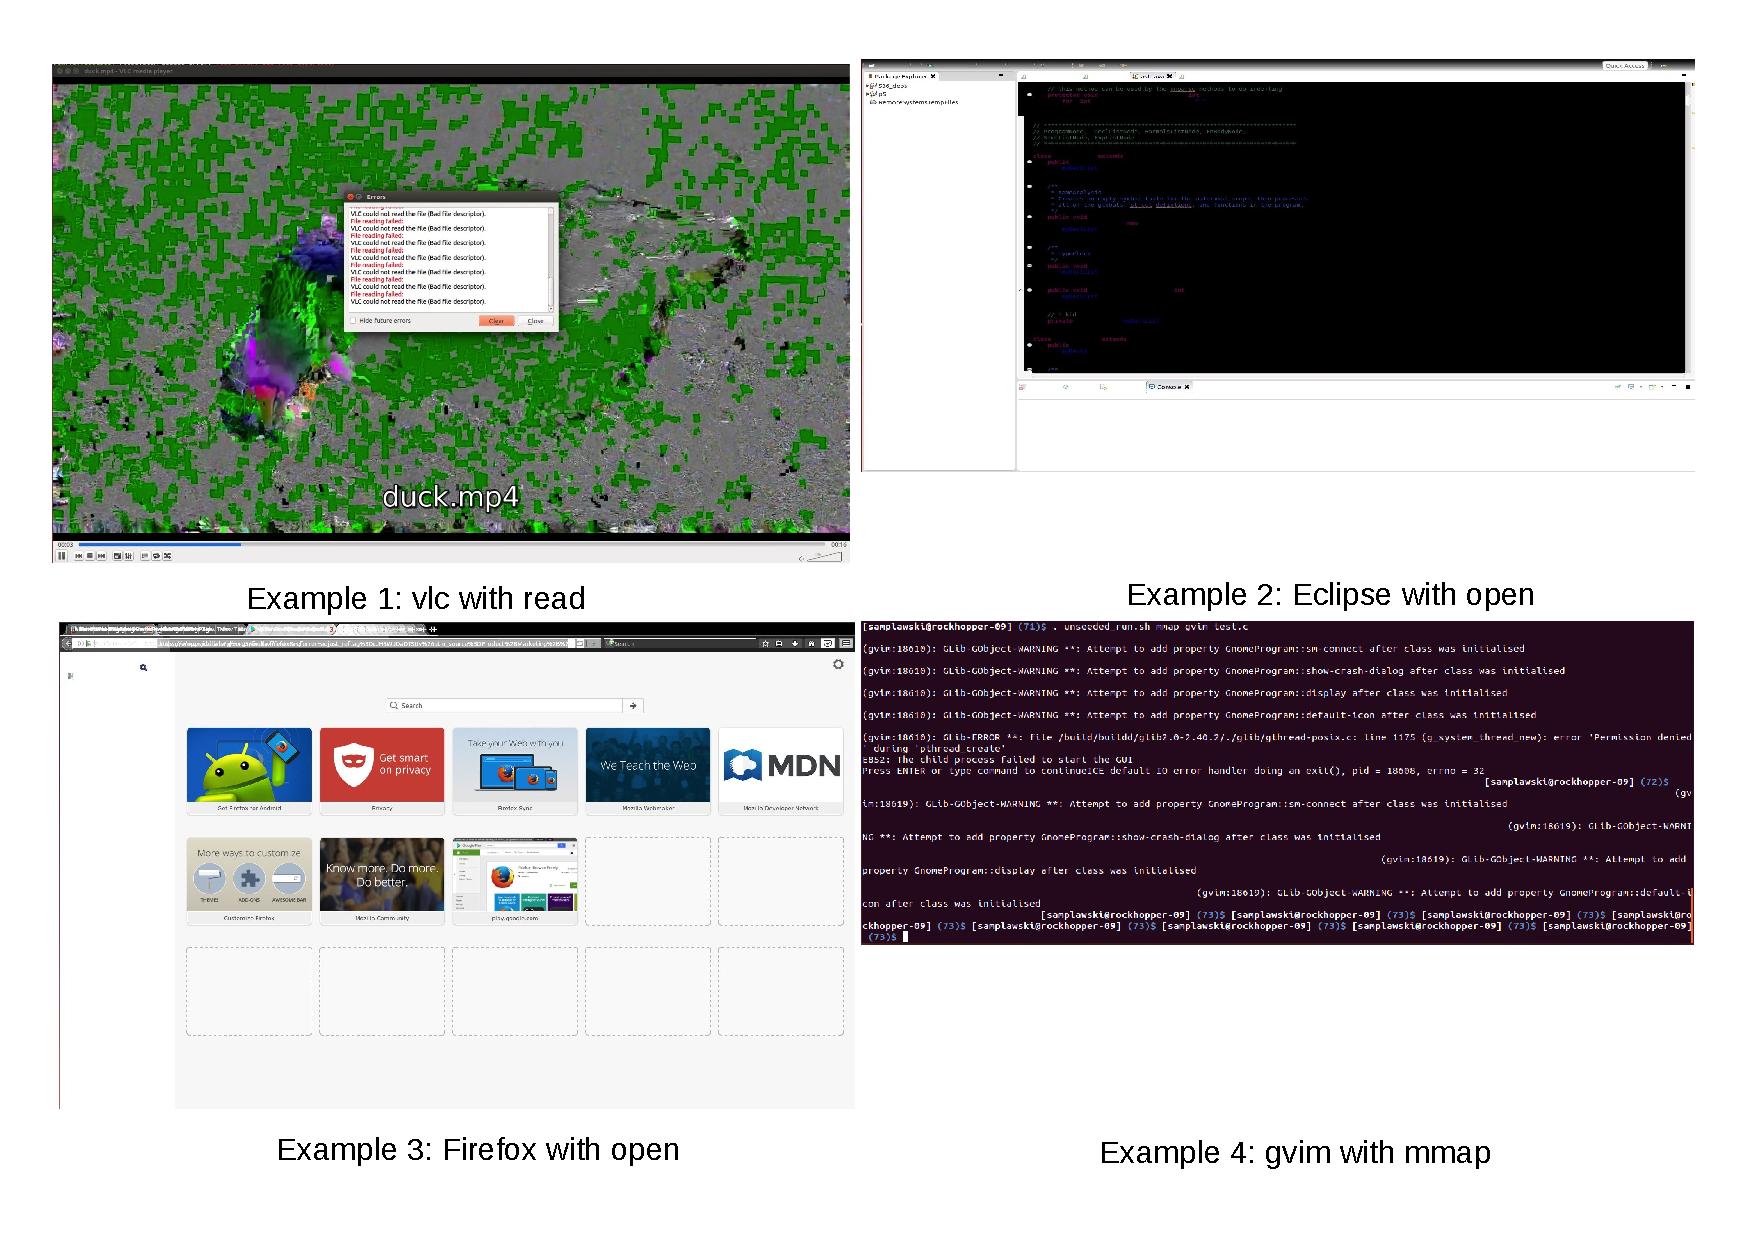
\includepdf[scale=.8, angle=90, pagecommand=\section{Anecdote Examples}]{an.pdf}

\end{document}
